\chapter{O que a margem deixa de fora}\label{cap:margem}

Este é o último pedaço do andar, e ele junta duas coisas que a espiral encontrou separadas: o vigia
de margem não vê o que acontece \textbf{entre} as pernas, e ler uma série pelo segundo momento é ler
metade dela. A pergunta é quanto custa a metade que fica de fora.

\section{O experimento controlado pelo segundo momento}

Para medir o que a margem não conta é preciso um par de mundos que tenha tudo igual e uma coisa
diferente. A família usada aqui tem a correlação \textbf{declarada}: com probabilidade $p$ as duas pernas
recebem o mesmo choque, de tamanho $f$, e a correlação do corpo é resolvida para que a correlação
total continue valendo \numMargemRho{} em todos os mundos. Nas linhas da tabela, o dois, o cinco e o dez
por cento nomeiam $p$ --- a chance de o choque comum acontecer ---, e o tamanho $f$ é o mesmo nos três:
o mundo do choque grande repete os cinco por cento com um choque maior.
% aterramento: f
O que muda de um mundo para o outro é a forma como os dias ruins chegam juntos --- e também o
tamanho de cada perna, que o choque comum engrossa: a variância da margem sobe de
\numMargemVarianciaMenor{} a \numMargemVarianciaMaior{} entre o controle e o mundo mais grosso.

O controle é o par gaussiano puro, que é o mundo sem choque comum. A família tem \numMargemMundos{} mundos --- o controle e
quatro com o choque declarado ---, medidos em \numMargemDias{} dias e
\numMargemSementes{} sorteios por célula, com o corte na janela de \numMargemJanela{} dias e a
carteira com peso igual, \numMargemPeso{} em cada perna.

Se o segundo momento resumisse o risco conjunto, nada mudaria entre esses mundos.

\section{O que fica parado e o que cresce}

\begin{table}[htbp]
  \centering
  \small
  \resizebox{\linewidth}{!}{%
\begin{tabular}{lrrr}
    \hline
    mundo & correlação & curtose da & dias juntos, \\
    & medida & margem & contra a independência \\
    \hline
    controle & \numMargemCorrelacaoControle & \numMargemCurtoseControle & \numMargemExcessoControle \\
    choque em dois por cento & \numMargemCorrelacaoDoisPorCento & \numMargemCurtoseDoisPorCento & \numMargemExcessoDoisPorCento \\
    choque em cinco por cento & \numMargemCorrelacaoCincoPorCento & \numMargemCurtoseCincoPorCento & \numMargemExcessoCincoPorCento \\
    choque em dez por cento & \numMargemCorrelacaoDezPorCento & \numMargemCurtoseDezPorCento & \numMargemExcessoDezPorCento \\
    choque grande & \numMargemCorrelacaoChoqueGrande & \numMargemCurtoseChoqueGrande & \numMargemExcessoChoqueGrande \\
    \hline
  \end{tabular}}
  \caption{A correlação declarada é respeitada em todos os mundos --- a medida vai de
    \numMargemCorrelacaoMenor{} a \numMargemCorrelacaoMaior{} ---, e o que muda é a cauda e o
    agrupamento dos dias ruins. A última coluna é o instrumento do capítulo da dependência: quantas
    vezes os dois rompem juntos, contra o que a independência preveria.}
  \label{tab:margem}
\end{table}

A correlação anda de \numMargemCorrelacaoMenor{} a \numMargemCorrelacaoMaior{}, um vaivém de menos
de dois por cento que é ruído de amostragem. No mesmo conjunto de mundos, os dias em que as duas
pernas rompem juntas vão de \numMargemExcessoMenor{} a \numMargemExcessoMaior{} vezes o que a
independência preveria: quase o dobro. A \emph{correlação} fica parada enquanto o agrupamento dos dias
ruins quase dobra --- mas o segundo momento não fica: o choque comum engrossa cada perna, e a
variância da margem dobra. Duas contas separam a escala da forma. Padronizando cada perna pela própria
variância antes de medir a perda, a razão entre o pior mundo e o controle cai de \numMargemPerdaRazao{}
para \numMargemPerdaPadraoRazao. E uma gaussiana com a variância e a correlação de cada mundo --- sem
cauda nenhuma --- já entrega \numMargemPerdaGaussianaRazao{} dessa razão: \textbf{a maior parte do que
a perda conjunta cresce é a margem que o choque engrossou}, e o que sobra para a forma é a parte
pequena, que é a que este capítulo persegue.

\begin{table}[htbp]
  \centering
  \small
  \begin{tabular}{lrr}
    \hline
    mundo & perda conjunta & além do próprio \\
    & no pior \numMargemCauda{} & corte \\
    \hline
    controle & \numMargemPerdaControle & \numMargemProfundidadeControle \\
    choque em dois por cento & \numMargemPerdaDoisPorCento & \numMargemProfundidadeDoisPorCento \\
    choque em cinco por cento & \numMargemPerdaCincoPorCento & \numMargemProfundidadeCincoPorCento \\
    choque em dez por cento & \numMargemPerdaDezPorCento & \numMargemProfundidadeDezPorCento \\
    choque grande & \numMargemPerdaChoqueGrande & \numMargemProfundidadeChoqueGrande \\
    \hline
  \end{tabular}
  \caption{A perda média de uma carteira de peso igual no pior \numMargemCauda{} dos dias, e a
    profundidade média além do corte de uma das pernas. A coluna da perda é o prejuízo; a de além do corte é
    o que a margem paga quando ele é rompido.}
  \label{tab:perdas}
\end{table}

A perda conjunta sai de \numMargemPerdaMenor{} para \numMargemPerdaMaior{}, uma razão de
\numMargemPerdaRazao{} entre o mundo mais calmo e o mais pesado, sem que a correlação tenha se
mexido. Quem dimensiona a proteção pela correlação dimensiona o mesmo número para os cinco mundos, e
o que se paga no pior dia difere por mais da metade.

\begin{figure}[htbp]
  \centering
  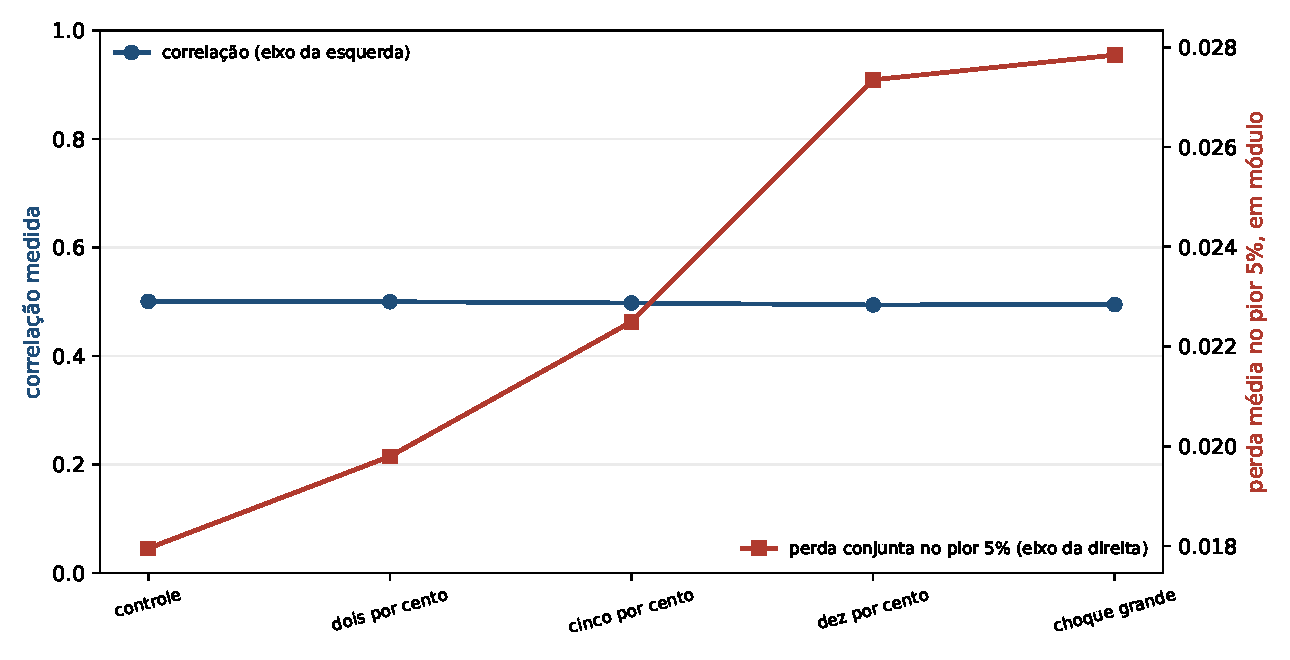
\includegraphics[width=\linewidth]{figuras/E17_o_que_a_margem_nao_conta_1.pdf}
  \caption{A correlação medida e a perda conjunta, contra os cinco mundos. Os dois eixos são
    diferentes de propósito, e as duas linhas se cruzam no meio do caminho: a reta é a correlação, que
    anda de \numMargemCorrelacaoMenor{} a \numMargemCorrelacaoMaior{}, e a que sobe é a perda, que
    começa abaixo dela e termina acima.}
  \label{fig:parado}
\end{figure}

\section{A margem cumpre a taxa e paga mais fundo}

Vale ser exato sobre o que a margem conta e o que ela não conta, porque a diferença é fina e importa.

A taxa de rompimento do corte é \numMargemTaxaDeRompimento{}, na média dos cinco mundos, e o motivo é do
instrumento: o corte é um quantil, e um quantil entrega a taxa que promete em qualquer mundo que tenha
uma distribuição contínua. A promessa do corte é honrada em todos eles.

O que não é honrado é o que acontece \textbf{depois} do rompimento. A profundidade média além do corte vai
de \numMargemProfundidadeControle{} no controle a \numMargemProfundidadeChoqueGrande{} no mundo de
choque grande: o dia em que o corte é rompido passa a doer três vezes e meia mais, e o número de dias não
mudou.
% aterramento: curtose
A curtose é a média da quarta potência da série depois de ela ter sido posta na própria unidade, e
vale três no mundo normal:
quanto maior, mais peso na cauda. A margem conta que a cauda engordou --- a curtose dela vai de \numMargemCurtoseMenor{} a
\numMargemCurtoseMaior{}, e isso é visível numa série só. O que ela não conta é que os dias
engordaram \textbf{juntos}.

\begin{figure}[htbp]
  \centering
  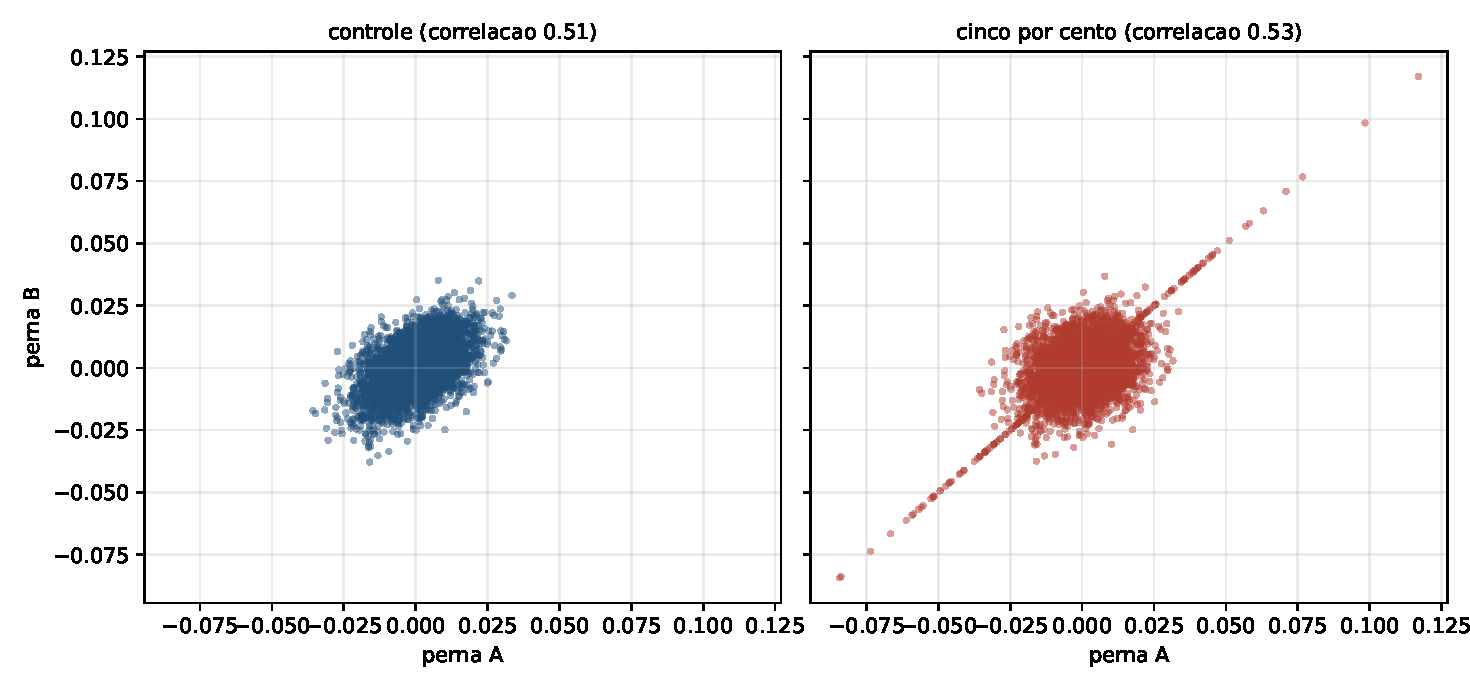
\includegraphics[width=\linewidth]{figuras/E17_o_que_a_margem_nao_conta_2.pdf}
  \caption{A nuvem das duas pernas no mundo gaussiano e no mundo com choque comum. O miolo se abre
    para que a correlação do conjunto continue a mesma, e o que o segundo tem a mais são dois braços
    na diagonal, um para cada canto.}
  \label{fig:nuvem-do-choque}
\end{figure}

Os braços são poucos pontos e ficam fora do corpo da nuvem, além da caixa em que quase todos os
pontos vivem. Um recorte na altura do miolo, que é o corte natural de quem desenha o que é comum,
apagaria exatamente o que o mundo do choque tem a mais.

A figura mostra a diferença de forma, e ela é a coisa toda. Nos dois mundos o miolo é quase a mesma
elipse, e é ele que teve de se abrir para que a correlação do conjunto continuasse em \numMargemRho{}.
O que o mundo do choque tem a mais são dois braços na diagonal, que saem do miolo e vão até os
cantos do gráfico, um para cima e outro para baixo: são os dias em que as duas pernas se movem
juntas e fundo, porque o choque comum tem sinal sorteado, e é no braço de baixo que o prejuízo mora.

\section{O que fica}

Fica a resposta do terceiro pedaço do andar, e ela é mais fina do que a queixa usual contra a
correlação \cite{koike2026measuring}. A margem \textbf{não} é cega à cauda: ela conta que a cauda engordou, e conta pela taxa e pela
profundidade. O que ela não conta é a \textbf{junto}; e como o prejuízo de uma carteira é feito de dias em
que tudo cai ao mesmo tempo, é justamente a parte que falta que decide a conta.

Fica também, com este capítulo, o andar inteiro medido. Os três pedaços são o mesmo movimento visto
de três lugares: o resumo --- o recorde, o estado guardado, o segundo momento --- é sempre uma
compressão, e o que escapa da compressão é exatamente o que decide. O mundo que faltou não está no
recorde, o dia apagado não está no estado, e o dia em que tudo cai junto não está na correlação.

A espiral vira agora para o andar do enquadramento. Tudo o que a espiral mediu até aqui supôs que
havia uma série, um agora e um sistema com fronteira --- e nenhuma dessas três coisas foi discutida.
Elas vêm a seguir, e vêm porque a conta deste andar mostrou quanto custa o que fica de fora quando a
fronteira é escolhida no escuro.
